

\subsection{Clusters}\label{sec:result:clusters}

\Warning[TODO]{ Rewrite this section! }

This is a simple clustering analysis of the datasets, clustered on a user basis.

The clustering algorithm used is k-means, operating on $U * S$ if $U * S * V'$ forms a rank $k$ SVD approximation of the interaction matrix $A$. The resulting rows in the matrix (the user ones) are then reordered and grouped with respect to their clusters.

This will try to group similar users next to each other. The used number of clusters is 10, this is not the optimal number of clusters for the datasets but the results are still useful for determining if there exists any clusters in the datasets.

Some of the graphs will be sparse and some will appear to be very dense. This is mostly due to resolution issues as when the dataset grow, even though the sparsity might be lower, the number of data points grow but the size of each data point in the graphs are the same.

\FloatBarrier

\twopic{fig/data/alphaS_original.png}{fig/data/alphaS_10-clusters.png}{
\textit{alphaS}
}

In \textit{alphaS} there are some clusters whith relatively few item interactions, but the other clusters aren't very prominent. Both \textit{alpha} and \textit{alpha2} are so large the resolution isn't enough to capture any individual data points so their graphs doesn't show anything of value so they are not included here.

\twopic{fig/data/eswc2015books_original.png}{fig/data/eswc2015books_10-clusters.png}{
\textit{eswc2015books}
}

\FloatBarrier

\textit{eswc2015books} doesn't seem to have any major clusters, the dataset doesn't appear to have any structure except for a few streaks of very popular items.

\FloatBarrier

\twopic{fig/data/eswc2015movies_original.png}{fig/data/eswc2015movies_10-clusters.png}{
\textit{eswc2015movies}
}

\twopic{fig/data/eswc2015music_original.png}{fig/data/eswc2015music_10-clusters.png}{
\textit{eswc2015music}
}

\textit{eswc2015movies} and \textit{eswc2015music} in contrast display more prominent clusters. There are clusters who concentrate more on a subset of items, and there are clusters with higher interaction count.  Similarly \textit{movielens1m} and \textit{romeo} also have distinct clusters.

\twopic{fig/data/movielens1m_original.png}{fig/data/movielens1m_10-clusters.png}{
\textit{movielens1m}
}

\twopic{fig/data/romeo_original.png}{fig/data/romeo_10-clusters.png}{
\textit{romeo}
}

\FloatBarrier

\twodiffpic{fig/data/alphaS_10-clusters_item_sorted.png}{\textit{alphaS}}
{fig/data/eswc2015books_10-clusters_item_sorted.png}{\textit{eswc2015books}}

\twodiffpic{fig/data/eswc2015movies_10-clusters_item_sorted.png}{\textit{eswc2015movies}}
{fig/data/eswc2015music_10-clusters_item_sorted.png}{\textit{eswc2015music}}

\twodiffpic{fig/data/movielens1m_10-clusters_item_sorted.png}{\textit{movielens1m}}
{fig/data/romeo_10-clusters_item_sorted.png}{\textit{romeo}}

\FloatBarrier

\newpage

\subsection{Spectral clustering}

k-means cluster for compactness while spectral clustering cluster based on connectivity.

\url{https://charlesmartin14.wordpress.com/2012/10/09/spectral-clustering/}

The basic steps are as follows:

\begin{enumerate}
    \item Create an affinity matrix, or simpler an adjacency matrix, $A_{f}$
    \item Construct a Graph Laplacian $L$
    \item Find eigenvalues and eigenvectors of $L$
    \item Select a subspace of eigenvectors
    \item Form clusters in the subspace
\end{enumerate}

In our particular case, the interaction matrix $A$ is defined as rows corresponding to users and columns corresponding to items. The affinity matrix needs to be square, but the interaction matrix is not. There are other more complex ways of creating an affinity matrix, but for this purpose modelling a simple adjacency matrix is sufficient.
\Warning[TODO]{ What complex ways? }

A transformation from the interaction matrix $A$ to the adjacency matrix $A_{f}$ is made by having both users and items as both row and column indices and mirroring the interactions. $A_{f}$ will then be a symmetric, square matrix. \eqref{eq:make_adj} illustrates an example.

\begin{equation}\label{eq:make_adj}
  A = \kbordermatrix{
    &    i_1 & i_2 & i_3 & i_4 \\
    u_1 & 0   & 1   & 0   & 1  \\
    u_2 & 0   & 1   & 1   & 1  \\
    u_3 & 1   & 0   & 1   & 0
  }
  \Rightarrow
    A_f = \kbordermatrix{
        &    u_1 & u_2 & u_3 & i_1 & i_2 & i_3 & i_4 \\
        u_1 & 0   & 0   & 0  &  0  &  1  &  0  &  1  \\
        u_2 & 0   & 0   & 0  &  0  &  1  &  1  &  1  \\
        u_3 & 0   & 0   & 0  &  1  &  0  &  1  &  0 \\
        i_1 & 0   & 0   & 1  &  0  &  0  &  0  &  0 \\
        i_2 & 1   & 1   & 0  &  0  &  0  &  0  &  0 \\
        i_3 & 0   & 1   & 1  &  0  &  0  &  0  &  0 \\
        i_4 & 1   & 1   & 0  &  0  &  0  &  0  &  0 \\
    }
\end{equation}

\begin{figure}[h!]
    \begin{subfigure}[h!]{0.5\textwidth}
        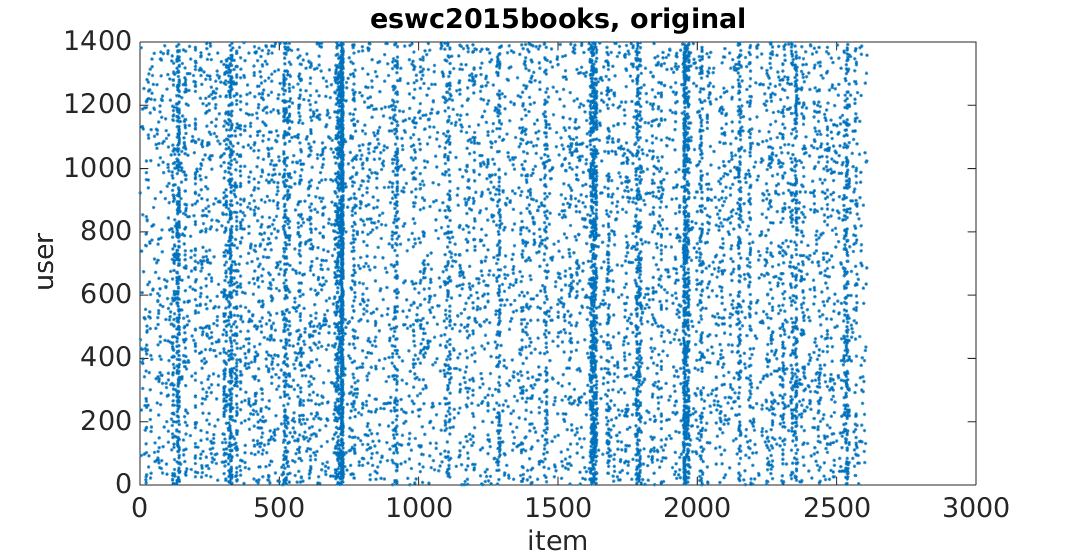
\includegraphics[width=\textwidth]{fig/spectral_data/eswc2015books_original.png}
        \caption{Interaction matrix $A$}
        \label{fig:spec:book:orig}
    \end{subfigure}
    ~
    \begin{subfigure}[h!]{0.5\textwidth}
        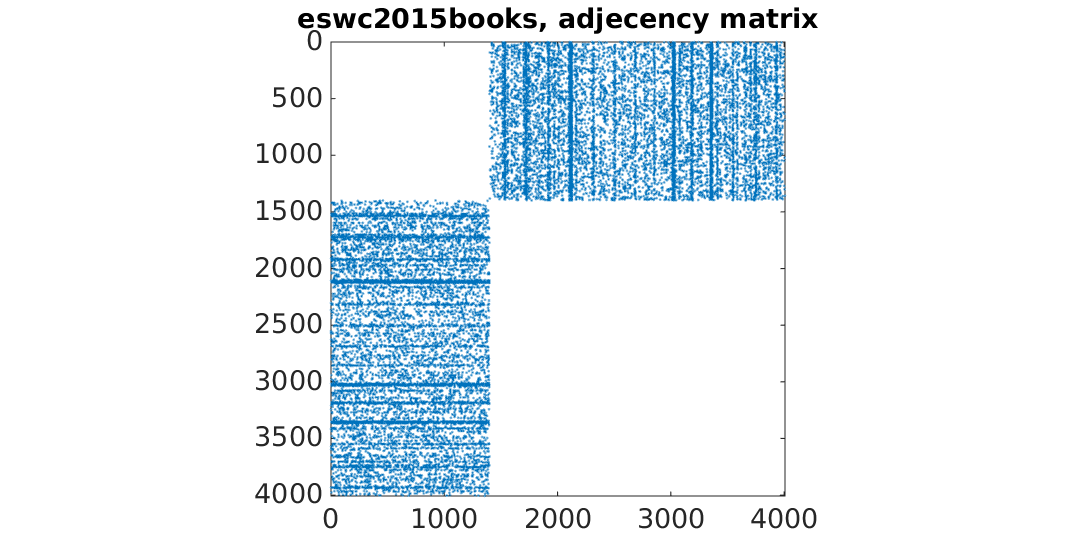
\includegraphics[width=\textwidth]{fig/spectral_data/eswc2015books_adj.png}
        \caption{Adjacency matrix $A_f$}
        \label{fig:spec:book:adj}
    \end{subfigure}
    \caption{This figure illustrates the original interaction matrix \ref{fig:spec:book:orig} for \textit{eswc2015books} and the related adjecency matrix \ref{fig:spec:book:adj}. Here the matrix $A$ has been moved to the upper right corner of $A_f$ as well as mirrored at the bottom left.}
\end{figure}

There are different kinds of Laplacians in literature, the one used here is the simple Laplacian $L = D - A_f$ where $D$ is a diagonal matrix called the degree matrix, representing the sum of the degrees at each node $i$:
\Warning[TODO]{ Ref needed! }

\begin{equation}
    D_{i, i} = \sum_j a_{i, j}
\end{equation}

The principal idea is that if good clusters can be identified, then the Laplacian $L$ is approximately block diagonal, with each cluster defined by a block. That is if there are 3 clusters

\begin{equation}
    \begin{pmatrix}
        L_{1, 1} & L_{1, 2} & L_{1, 3} \\
        L_{2, 1} & L_{2, 2} & L_{2, 3} \\
        L_{3, 1} & L_{3, 2} & L_{3, 3}
    \end{pmatrix}
    \sim
    \begin{pmatrix}
        L_{1, 1} & 0         & 0        \\
        0        & L_{2, 2}  & 0        \\
        0        & 0         & L_{3, 3}
    \end{pmatrix}
\end{equation}

Then also the lowest eigenvalues and their related eigenvectors correspond to different clusters. In this case the 3 smallest eigenvalues and eigenvector pair would correspond to each cluster, or block, in $L$.

To be able to identify different clusters, the sorted eigenvalues must have a gap. \Figureref{fig:spec:book:eigv} give a concrete example for \textit{eswc2015books}. It is reasonable to expect there to be 4 clusters in the adjacency matrix $A_f$. Note that this doesn't mean that there are as many clusters in the interaction matrix $A$, as there is duplicate information in $A_f$. There might be large areas without interactions, but the indexes might correspond to user-user or item-item which will not have any interactions.

The subspace to find clusters in is some subset of the eigenvectors corresponding to the smallest eigenvalues. The subspaced used here is simply the eigenvector corresponding to the 2nd smallest eigenvalue. \Figureref{fig:spec:book:eigsort} displays the adjacency matrix $A_f$ for \textit{eswc2015books} ordered by the ordering used when sorting the subspace. There might be some clustering visible, one small square to the top left end one larger square at the bottom right, but it's hard to identify.

\FloatBarrier

\twodiffpiclabel{fig/spectral_data/eswc2015books_eigv.png}
{The smallest eigenvalues of $L$ for \textit{eswc2015books}.}
{fig:spec:book:eigv}
{fig/spectral_data/eswc2015books_eig_sort.png}
{Adjacency matrix $A$ of \textit{eswc2015books}, sorted by the reordering used when sorting the 2nd smallest eigenvector of $L$.}
{fig:spec:book:eigsort}

\FloatBarrier

If instead of simply sorting the subspace, \textit{k-means} is used to find a clustering in the subspace, and that ordering is then used to reorder the adjacency matrix. \Figureref{fig:spec:book:kmeans} displays the adjacency matrix $A_f$ received for \textit{eswc2015books}. There are several, very clear, clusters visible. The same clustering information was used to reveal clusters in
the original interaction matrix $A$, visible in \figureref{fig:spec:book:clust}.

\FloatBarrier

\twodiffpiclabel{fig/spectral_data/eswc2015books_kmeans_sort.png}
{Adjacency matrix $A_f$ of \textit{eswc2015books}, subspace clustered with \textit{k-means}.}
{fig:spec:book:kmeans}
{fig/spectral_data/eswc2015books_spectral_clust.png}
{Interaction matrix $A$ of \textit{eswc2015books}, reordered using \textit{k-means} clustering information.}
{fig:spec:book:clust}

\FloatBarrier

What follows is a similar analysis for other datasets.

\FloatBarrier

\twodiffpiclabel{fig/spectral_data/alphaS_eigv.png}
{The smallest eigenvalues of $L$ for \textit{alphaS}.}
{fig:spec:alphaS:eigv}
{fig/spectral_data/alphaS_eig_sort.png}
{Adjacency matrix $A$ of \textit{alphaS}, sorted by the subspace ordering.}
{fig:spec:alphaS:eigsort}

\twodiffpiclabel{fig/spectral_data/alphaS_kmeans_sort.png}
{Adjacency matrix $A_f$ of \textit{alphaS}, subspace clustered with \textit{k-means}.}
{fig:spec:alphaS:kmeans}
{fig/spectral_data/alphaS_spectral_clust.png}
{Interaction matrix $A$ of \textit{alphaS}, reordered using \textit{k-means} clustering information.}
{fig:spec:alphaS:clust}

\FloatBarrier

\textit{alphaS} have many clusters which is evident in the clustered interaction matrix in \figureref{fig:spec:alphaS:clust}. This is supported by the large number of small eigenvalues in \figureref{fig:spec:alphaS:eigv} preceeding a gap and also visible even without resorting to clustering but simply sorting the subspace in \figureref{fig:spec:alphaS:eigsort}.

\FloatBarrier

\twodiffpiclabel{fig/spectral_data/eswc2015movies_eigv.png}
{The smallest eigenvalues of $L$ for \textit{eswc2015movies}.}
{fig:spec:eswc2015movies:eigv}
{fig/spectral_data/eswc2015movies_eig_sort.png}
{Adjacency matrix $A$ of \textit{eswc2015movies}, sorted by the subspace ordering.}
{fig:spec:eswc2015movies:eigsort}

\twodiffpiclabel{fig/spectral_data/eswc2015movies_kmeans_sort.png}
{Adjacency matrix $A_f$ of \textit{eswc2015movies}, subspace clustered with \textit{k-means}.}
{fig:spec:eswc2015movies:kmeans}
{fig/spectral_data/eswc2015movies_spectral_clust.png}
{Interaction matrix $A$ of \textit{eswc2015movies}, reordered using \textit{k-means} clustering information.}
{fig:spec:eswc2015movies:clust}

\FloatBarrier

There might be some clustering in \textit{eswc2015movies}, maybe in the top right corner in \figureref{fig:spec:eswc2015movies:clust}, but the plots are not very clear. The reason it looks like there are clear clusters in \figureref{fig:spec:eswc2015movies:kmeans} is the large difference between the number of users and the number of items and the white space are simple item-item or user-user which never have any interactions between them.

\textit{eswc movies/music movielens might do with only eigenvalues and final matrix!}

\FloatBarrier

\twodiffpiclabel{fig/spectral_data/eswc2015music_eigv.png}
{The smallest eigenvalues of $L$ for \textit{eswc2015music}.}
{fig:spec:eswc2015music:eigv}
{fig/spectral_data/eswc2015music_eig_sort.png}
{Adjacency matrix $A$ of \textit{eswc2015music}, sorted by the subspace ordering.}
{fig:spec:eswc2015music:eigsort}

\twodiffpiclabel{fig/spectral_data/eswc2015music_kmeans_sort.png}
{Adjacency matrix $A_f$ of \textit{eswc2015music}, subspace clustered with \textit{k-means}.}
{fig:spec:eswc2015music:kmeans}
{fig/spectral_data/eswc2015music_spectral_clust.png}
{Interaction matrix $A$ of \textit{eswc2015music}, reordered using \textit{k-means} clustering information.}
{fig:spec:eswc2015music:clust}

\FloatBarrier

\twodiffpiclabel{fig/spectral_data/movielens1m_eigv.png}
{The smallest eigenvalues of $L$ for \textit{movielens1m}.}
{fig:spec:movielens1m:eigv}
{fig/spectral_data/movielens1m_eig_sort.png}
{Adjacency matrix $A$ of \textit{movielens1m}, sorted by the subspace ordering.}
{fig:spec:movielens1m:eigsort}

\twodiffpiclabel{fig/spectral_data/movielens1m_kmeans_sort.png}
{Adjacency matrix $A_f$ of \textit{movielens1m}, subspace clustered with \textit{k-means}.}
{fig:spec:movielens1m:kmeans}
{fig/spectral_data/movielens1m_spectral_clust.png}
{Interaction matrix $A$ of \textit{movielens1m}, reordered using \textit{k-means} clustering information.}
{fig:spec:movielens1m:clust}

\FloatBarrier

\textit{movielens1m} has some distinct clusters, visible in \figureref{fig:spec:movielens1m:clust}. The large eigenvalue gap in \figureref{fig:spec:movielens1m:eigv} supports this finding.

\FloatBarrier

\twodiffpiclabel{fig/spectral_data/romeo_eigv.png}
{The smallest eigenvalues of $L$ for \textit{romeo}.}
{fig:spec:romeo:eigv}
{fig/spectral_data/romeo_eig_sort.png}
{Adjacency matrix $A$ of \textit{romeo}, sorted by the subspace ordering.}
{fig:spec:romeo:eigsort}

\twodiffpiclabel{fig/spectral_data/romeo_kmeans_sort.png}
{Adjacency matrix $A_f$ of \textit{romeo}, subspace clustered with \textit{k-means}.}
{fig:spec:romeo:kmeans}
{fig/spectral_data/romeo_spectral_clust.png}
{Interaction matrix $A$ of \textit{romeo}, reordered using \textit{k-means} clustering information.}
{fig:spec:romeo:clust}

\FloatBarrier

\newpage
